\documentclass[25pt,a0paper,portrait]{tikzposter}

\usepackage[utf8]{inputenc}
\usepackage[T1]{fontenc}
\usepackage{xcolor}
\usepackage{graphicx}
\usepackage{tikz}
\usepackage{multicol}
\usepackage{adjustbox}
\usepackage{booktabs}
\usepackage{comment}

\setlength{\itemsep}{2pt}

\makeatletter
\def\TP@titlegraphictotitledistance{-6cm}
\settitle{%
	\centering
	\vbox{%
		\@titlegraphic\\[\TP@titlegraphictotitledistance]
		\centering\color{titlefgcolor}%
		{\bfseries\Huge\scshape \@title\par}%
		\vspace*{1em}%
		{\huge \@author\par}%
	}%
}
\makeatother

\setlength{\columnsep}{2cm}

% Metadata
\title{Sales Forecasting for Walmart}
\author{Adil Ibraheem Koyava, Ayush Plawat,\\Hemanth Jadiswami Prabhakaran }

\titlegraphic{%
	
\includegraphics[height=6.5cm]{images/HochschuleLogo}\hfill
	
\includegraphics[height=6.5cm]{images/logo2.jpeg}%
}

\usetheme{Desert}

\begin{document}
	\maketitle
	
	\begin{columns}
		
		% ===================== LEFT COLUMN =====================
		\column{0.5}
		\colorlet{blocktitlebgcolor}{blue}
		
		\block{Problem Description}{
			\textbf{Retail Forecasting Complexity:}
			Walmart operates 45 U.S. stores with 81 departments, each experiencing complex seasonal, regional, and promotional sales fluctuations. Traditional forecasting methods struggle with the complexity of multiple variables affecting weekly sales patterns.
			
			
			\textbf{Week-over-Week Prediction Challenge:}
			The system must predict weekly sales changes rather than absolute values, accounting for holiday effects, markdown promotions, and macroeconomic indicators across diverse store types and departments.
			
			
			\textbf{Data Integration Requirements:}
			Integration of three distinct datasets (sales history from train.csv, external features from features.csv, and store characteristics from stores.csv) with missing values, outliers, and non-stationary behavior requiring sophisticated preprocessing and modeling approaches.
	
		}
		
		\block{Data Overview}{
			\textbf{Sources:}
			\begin{itemize}
				\item \textbf{Sales:} Weekly sales per store-department from 2010–2012.
				\item \textbf{Store Info:} Store type (A/B/C) and size.
				\item \textbf{External:} Fuel price, temperature, CPI, unemployment, 5 MarkDowns (sparse).
			\end{itemize}
			
			\textbf{Findings:}
			Holiday spikes (especially Thanksgiving), high sales variance in Type A stores, and weak correlation with macroeconomic indicators.
			
			\begin{center}
				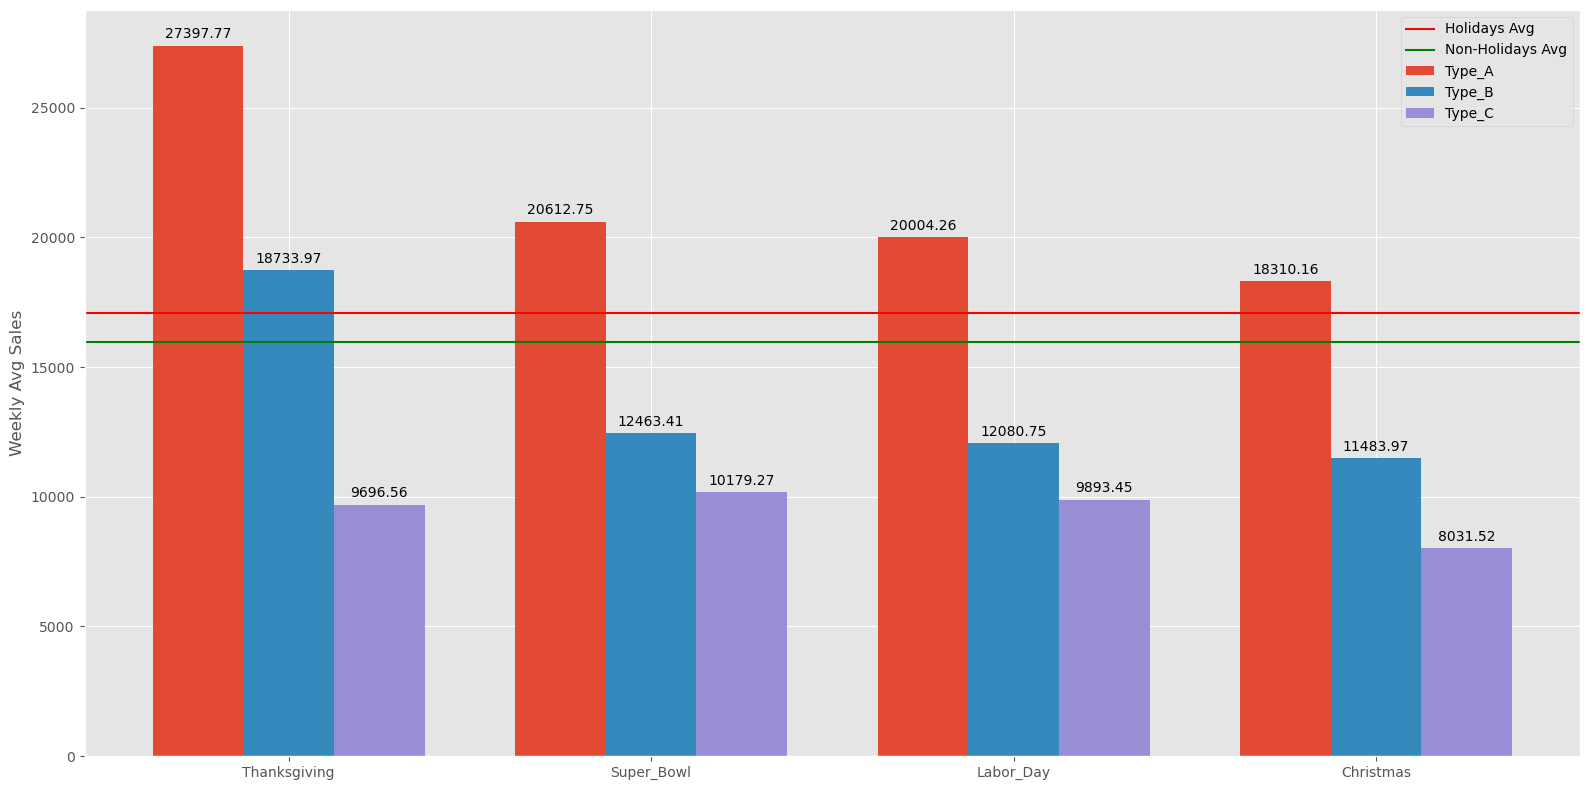
\includegraphics[width=0.8\linewidth]{images/HolidaySales.png}
			\end{center}
		}
		
		\block{Challenges}{
			\textbf{Data Quality Issues:}
			\begin{itemize}
				\item Missing values in promotional markdown columns requiring zero-imputation strategies.
				\item Outliers due to holiday shopping peaks necessitating 99th percentile clipping.
				\item Non-stationary behavior from promotional campaigns and seasonal variations.
			\end{itemize}
			
			\textbf{Technical Complexity:}
			\begin{itemize}
				\item Holiday effects vary significantly across 45 stores and 81 departments creating sparse store-department combinations.
				\item Seasonal cycle detection and optimization requiring 20-week period analysis with automated parameter selection.
				\item Week-over-week change prediction complexity versus absolute value forecasting requiring specialized algorithms.
				\item Integration of heterogeneous external features with varying predictive power for sales forecasting.
			\end{itemize}
		}
		
		\block{Solutions}{
			\textbf{Data Preprocessing Solutions:}
			\begin{itemize}
				\item Comprehensive data cleaning pipeline merging train.csv, features.csv, and stores.csv with automated schema validation.
				\item Strategic missing value imputation with domain knowledge and outlier management using 99th percentile clipping.
				\item Feature engineering including time-based features (WeekOfYear, Quarter, DayOfYear) and one-hot encoded holidays and store types.
			\end{itemize}
			
			\textbf{Advanced Modeling Approach:}
			\begin{itemize}
				\item Auto ARIMA with pmdarima 2.0.4 for automated parameter optimization and seasonal component detection.
				\item Exponential Smoothing (Holt-Winters) with triple smoothing components and systematic hyperparameter tuning.
				\item 20-week seasonal period optimization capturing retail seasonality patterns.
			\end{itemize}
			
		
			
		}
		

		
		% ===================== RIGHT COLUMN =====================
		\column{0.5}
		\colorlet{blocktitlebgcolor}{blue}
		
		\block{Results}{
			\textbf{Model Performance Comparison (WMAE Metrics):}
			
			\begin{center}
				\begin{tabular}{lcc}
					\toprule
					\textbf{Algorithm} & \textbf{Absolute WMAE} & \textbf{Normalized WMAE} \\
					\midrule
					Exponential Smoothing & 923.12 & \textbf{3.58\%} \\
					Auto ARIMA & 1\,156.8 & 4.12\% \\
					\bottomrule
				\end{tabular}
			\end{center}
			
			\textbf{Performance Achievements:}
			The Exponential Smoothing (Holt-Winters) model achieved excellent performance with 3.58\% normalized WMAE, categorized as "Excellent" for business forecasting applications (threshold < 5\%). This enables reliable stock management, staffing optimization, and promotion timing decisions.
			
			\textbf{Feature Importance Analysis:}
			The model effectively captured critical predictive patterns including 20-week seasonal optimization cycles, holiday impact (especially Thanksgiving), store type classifications (A, B, C), and consistent week-of-year patterns. Macroeconomic indicators showed limited correlation with weekly sales changes.
			

		}
		
		\block{System Implementation}{
			\textbf{Dual-Application Architecture:}
			\begin{itemize}
				\item Training Application (Port 8501) for model development and evaluation using Python 3.12 environment
				\item Prediction Application (Port 8502) for production-ready forecasting with pre-trained models
				\item Cross-platform deployment supporting both local installation and cloud access via Streamlit Community Cloud
			\end{itemize}
			
			\textbf{Technical Capabilities:}
			\begin{itemize}
				\item 4-week forecast horizon with reliable accuracy and consistent trend capture
				\item Interactive visualizations with positive/negative change indicators and export capabilities (CSV/JSON)
				\item Comprehensive model management with .pkl serialization format
			\end{itemize}
			
			\begin{center}
				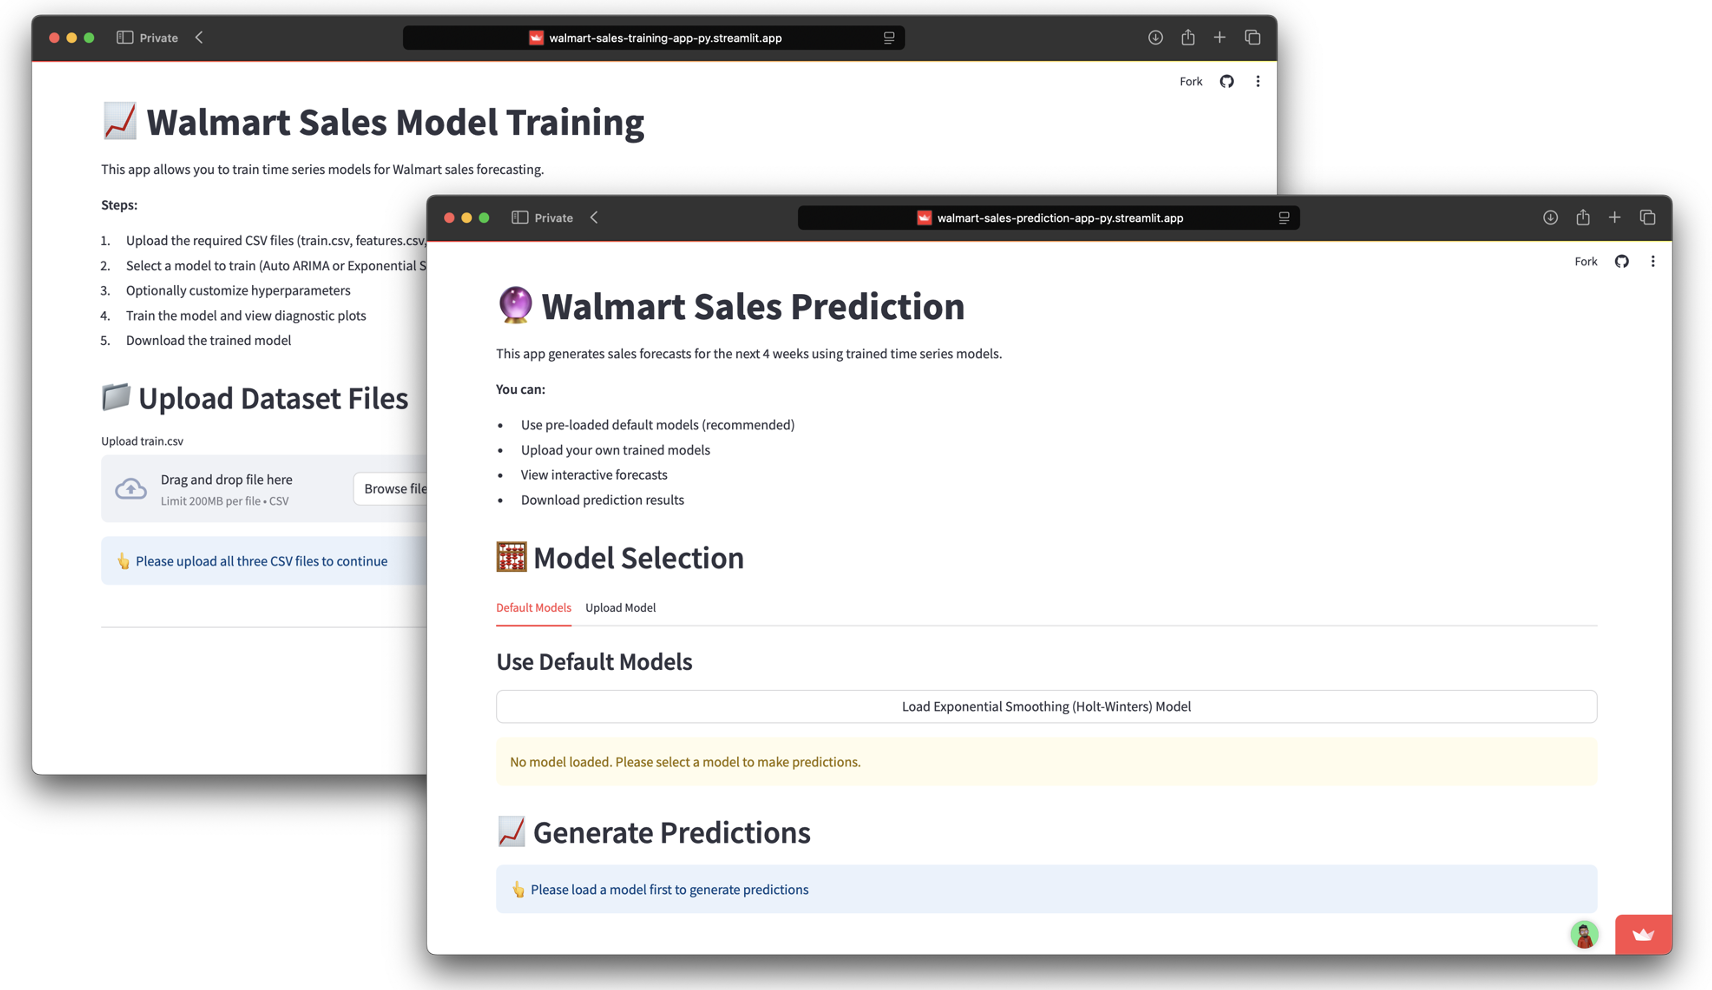
\includegraphics[width=0.7\linewidth]{images/result.png}
			\end{center}
		}
		
		\block{Business Impact \& Future Work}{
			\textbf{Practical Applications:}
			\begin{itemize}
				\item Actionable 4-week forecasts of week-over-week sales changes with positive values indicating sales increases and negative values representing decreases
				\item Enhanced decision support for retail operations planning and resource allocation
				\item Academic research tool for time series analysis learning and business analytics education
			\end{itemize}
			
			\textbf{Future Enhancements:}
			\begin{itemize}
				\item Extension of forecast horizon beyond current 4-week limitation with enhanced accuracy validation
				\item Implementation of ensemble methods combining multiple forecasting algorithms for improved robustness
				\item Integration of real-time data feeds and automated model updating capabilities
				\item Development of mobile application interface and enhanced accessibility features
			\end{itemize}
		}
		
		\block{Application QR Codes \& Data Set Links}{
			
				\begin{center}
				
\includegraphics[width=0.6\linewidth]{images/StaticQR.png}
			\end{center}
			
			
		}
		
	\end{columns}
\end{document}
